% !TEX root = thesis.tex
\chapter{深層学習の成果とアルゴリズム}
Deep Learningは、多層ニューラルネットワーク(MLP)のうち、普通隠れ層が2つ以上のものをいう。2006年にHintonらによって、このようなDeepな構造を学習させる方法が発見され、発展への道が開けた\cite{hinton2006a-fast, hinton2006reducing}。従来よりも多くのレイヤーを扱うことで、より複雑な関数を学習できるようになった。Deep Learningは、数々の分類タスクにて、従来手法を大きくしのぐ成果を収め、注目を浴びている。この章では、Deep Learningで使われているアルゴリズムの詳細について述べる。
\section{Deep Learningの成果}
第1章でも触れたが、2012年には、GoogleがYoutubeビデオの静止画を使って多層ニューラルネットワークの教師なし学習を行わせ、結果として、猫を認識するユニットや人を認識するユニットを学習させることに成功した。また、ImageNet Large Scale Visual Recognition Competition(ILSVRC)というデータセット\cite{deng2009imagenet:}の分類にて、state of the artの結果を残した。ImageNet\footnote{\url{http://www.image-net.org/}}とは、WordNet\footnote{\url{http://wordnet.princeton.edu/}}を真似して作られたデータセットである。2009年より、100を超える様々な論文にて、画像認識のベンチマークに利用されてきている\footnote{\url{http://www.image-net.org/about-publication}}。図\ref{c3_imagenet}は、ImageNetの画像の例である。画像はツリー状に分類されており、例えば上を見ると、mammal(哺乳類)→palcental(胎盤)→carnivore(肉食)→canine(イヌ科)→dog(イヌ)→working dog(盲導犬やそり犬など使役される犬)→husky(ハスキー)というように、徐々に分類が細かくなっていくことがわかる。また、一つのカテゴリーには、9枚の画像がひもづけられている。\par
\begin{figure}[tbp]
 \begin{center}
  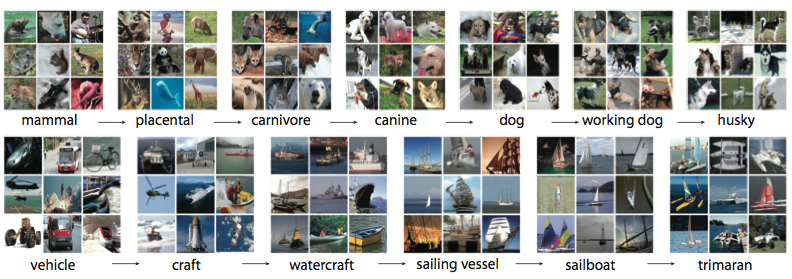
\includegraphics[width=120mm]{img/c3/imagenet}
 \end{center}
 \caption{Imagenetの画像とラベル構造の例}
 \label{c3_imagenet}
\end{figure}
Googleのsupervisionによる、画像分析の結果の例を図\ref{c3_supervision}に載せる(\cite{krizhevsky2012imagenet}より引用)。画像の分類に失敗している場合でも、妥当なラベルをつけていることがわかる。\begin{figure}[tbp]
 \begin{center}
  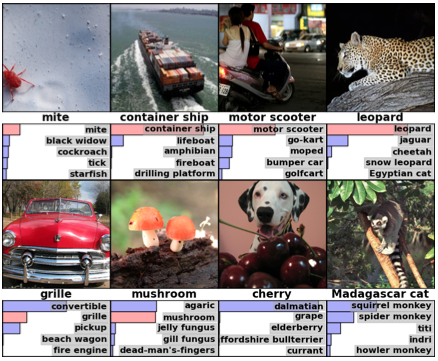
\includegraphics[width=80mm]{img/c3/supervision}
 \end{center}
 \caption{Supervisionによる画像分類の結果の例}
 \label{c3_supervision}
\end{figure}

\section{Deep Learningのアルゴリズム}
\subsection{Deep Belief Network}
最初にMLPの学習のブレイクスルーとなったのは、2006年のHintonらによるDeep Belief Nets(DBN)\cite{hinton2006a-fast, hinton2006reducing}である。このモデルについて解説する。
\subsubsection{unsupervised pretrainingとfinetuning}
この研究では、MLPの重みをランダムに初期化した後、すぐバックプロパゲーション学習にかけるのではなく、各レイヤーの重みをあらかじめ教師無し(unsupervised)学習で調整して、隠れ層が効率の良い素性を学習できるよう仕込んでおくというアイデアが使われた。この事前学習のことを、pretrainingと呼び、バックプロパゲーションにて学習する段階の方は、finetuningと呼ぶ。pretrainingの段階では、入力側から1レイヤーずつ学習を行い、学習済のレイヤーは固定して動かさない(Greedy Layer-wise pretraining)。finetuningの段階では、全てのレイヤーをバックプロパゲーションにて同時に変化させていく。DBNの構造を、図\ref{c3_dbn}に示す。\par
\begin{figure}[tbp]
 \centering
  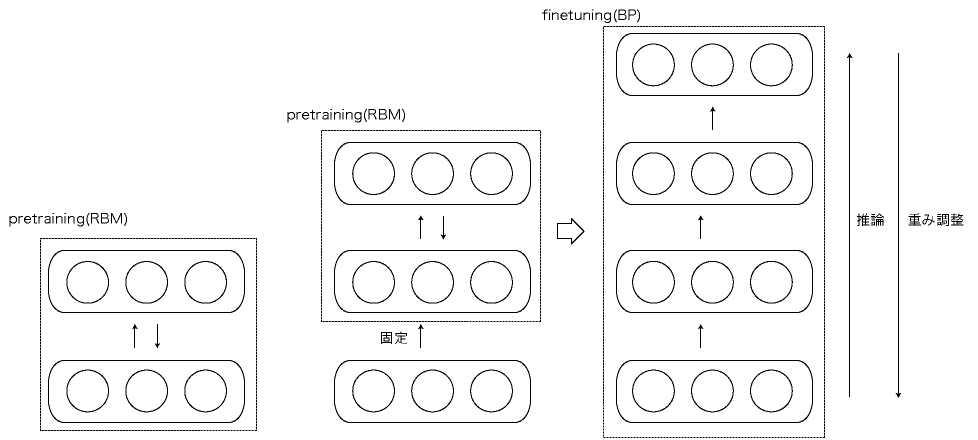
\includegraphics[width=120mm]{img/c3/dbn}
 \caption{Deep Belief Networkの構造と、学習過程}
 \label{c3_dbn}
\end{figure}
unsupervised pretrainingをどのような基準で行うかが問題だが、この研究では、Restricted Boltzman Machine(以下RBM)というモデルを用いている。RBMとは、ニューラルネットワークの一種で、可視変数層と隠れ変数層の2つのレイヤーから成り立っている。DBNにおいては、可視変数=入力データと考えておけばよい。RBMモデルの学習を進めることで、入力データ→隠れ変数への推論モデルを得ることができる。これがDeep Learningの最大の特徴の1つである、「抽象度の高い素性への変換方法自体を学習する」ことに対応している。DBNでは、RBMを1レイヤーずつ学習させながら、RBM同士を「前のレイヤーの隠れ層 = 次のレイヤーの入力層」となるようにつなげていく。これにより「入力層→抽象度の低いレイヤー→...→抽象度の高いレイヤー→出力」という、複数の隠れ層をもつDeepな構造を作り、上手くpretrainingさせることに成功している。RBMを積み重ねた最も上のレイヤーに、普通の線形レイヤーを1つ置いて、「最も抽象度の高い素性→出力値」の推測を行わせることが多い。なお、finetuningにおけるバックプロパゲーションでは、RBMにあった「隠れ層→入力層」の方のつながりは、最終レイヤーにおける誤差に影響しない。よって、以前からあるfeed-forwardなMLPと同様に学習させることができる。
\subsubsection{Restricted Boltzman Machine}
DBNのpretrainingに用いられるRestricted Boltzman Machine\cite{smolensky1986information}とは、ニューラルネットワークを用いた生成モデルの一種である。まず生成モデルについて説明する。\par
クラス分類問題を確率的アプローチで解く方法は、生成モデル(generative model)と識別モデル(判別モデル、discriminative model)の2つに大別できる\cite{bishop2006pattern}\footnote{確率モデルを介さず、入力からクラスを得る識別関数を直接導くことも出来る。}。クラス分類問題では、まずクラス事後確率$p(C_k|x)$を各クラス$k$に対して求める。基本的には入力$x$に対して最もクラス事後確率が大きくなったクラスに分類することになる\footnote{医療における誤診断など、誤分類のタイプに応じて重要度が異なる場合、損失関数(loss function)を導入することもある。}。識別モデルでは、クラス事後確率$p(C_k|x)$のみを直接学習するのに対し、生成モデルでは、まずクラスの条件付き密度$p(x|C_k)$を学習する。これと、別途求めたクラスの事前確率$p(C_k)$を用いることで、クラス事後確率は
\begin{equation}
p(C_k|x) = \frac{p(x | C_k)p(C_k)}{p(x)} = \frac{p(x | C_k)p(C_k)}{\sum_{k}p(x | C_k)p(C_k)}
\end{equation}
によって求められる。これは、入力とクラスの同時確率$p(C_k, x)$を求めることと等価である。生成モデルの利点は、クラス分類のモデルだけでなく、入力データの性質に関する情報をも同時に得られる点にある。しかし、一般に識別モデルよりも複雑で困難な問題を解く必要が生じるため、常に生成モデルが用いられるわけではない。\par
\begin{figure}[tbp]
 \centering
  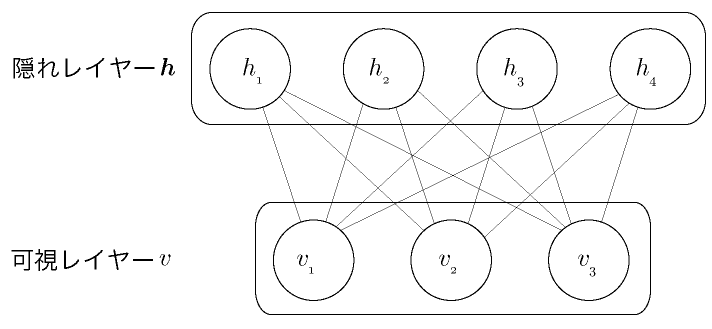
\includegraphics[width=100mm]{img/c3/rbm}
 \caption{Restriceted Boltzman Machineのネットワーク構造}
 \label{c3_rbm}
\end{figure}
さて、前述したように、RBMは可視層と隠れ層の2レイヤーで構成されるニューラルネットワークである。RBMの構造を、図\ref{c3_rbm}に示す。入力層の各ユニットの値を$v_j$, 隠れ層の各ユニットの値を$h_i$とおく。これらをまとめたベクトルをそれぞれ$\bm{v}=\{v_1, v_2, ...\}, \bm{h}=\{h_1, h_2, ...\}$とおく。これは、例えば$\bm{v}$が画像や音声などの入力データをベクトル化したもので、$\bm{h}$がこれらの変数の関係を説明する変数だと考えれば良い。ただし、$\bm{h}$が即$\bm{v}$のクラス分類に対応するとは限らないことに注意する。RBMの学習を進めると、$p(\bm{v}|\bm{h})$と$p(\bm{h}|\bm{v})$との、2方向の条件付き確率のモデルが同時に得られる。\par
RBMの学習は、自由エネルギーと呼ばれる従属変数を最小にするように行われる\footnote{自由エネルギーという呼び名は、物理学から採られている。}。ここでは、最も簡単かつ重要な、$v_j, h_i\epsilon\{0,1\}$のケースについて述べる。Wをvとhの間の重み、bとcを、それぞれvとhに対応するバイアス項とする。このとき、RBMにおける自由エネルギー$F(v)$は、
\begin{equation}
F(v) = -b' v-\sum_{i}log(1+e^{(c_i+W_{i}v)})
\end{equation}
となる。この自由エネルギーを、SGDなどのアルゴリズムを用いて最小化することで、目標となる生成モデルを得ることができる。なお、自由エネルギーの導入と最小化というアプローチは、Energy-Based Modelと呼ばれるアルゴリズム群に共通して用いられる概念であり、自由エネルギーにもさらに様々なモデルで使える一般的な定義が存在するが、割愛する。
\subsubsection{DBNの性能}
この研究では、評価実験としてMNISTの手書き数字認識データセットを用いている。彼らは各レイヤーのユニット数が"784-500-500-2000-10"という構造のDBNによって、学習を行った。そして、Permutation invariantと呼ばれるタスクにて、当時のstate fo the artを塗り替えたことにより、注目された。ここで、Permutation invariantとは、データを単なる1次元の値の集まりと見なし、2次元の画像という事前情報の利用を禁止した状態で、分類実験を行うことである。具体的には、画像的変形による水増しや、2次元的畳み込み(Convolutional Layerの節にて詳述)などが当てはまる。Permutation invariantの制約下で良い成果を出したDBNは、画像の性質を利用したConvolutional Netに比べたとき、画像以外の1次元のデータに対しても適用しやすいアルゴリズムだと考えられる。

\subsection{Stacked Denoising Autoencoder}
Deep Belief Networkと共に、1次元のデータに対して広く用いることができるモデルが、Stacked Denoising Autoencoderである。これは2007年に提唱されたStacked Autoencoder\cite{bengio2007greedy}というモデルを基に、2008年に発表された\cite{VincentPLarochelleH2008}。基本的なアイデアは、Deep Belief NetsにおけるRBMを、Denoising Autoencoderというモデルに変更することである。
\subsubsection{Autoencoder}
Denoising Autoencoderは、Autoencoderの特殊なバージョンなので、まずはAutoencoderについて説明する。Autoencoderは、ニューラルネットワークの一種であり、入力されたデータを再現するようなモデルを学習する。\cite{bourlard1988auto, hinton1994autoencoders, schwenk1995transformation}\par
Autoencoderの構造を、\ref{c3_autoencoder}に示す。Autoencoderは、この図でいうInput, Representation, Outputの3つのレイヤーから構成されている。OutputとInputの値が一致するように、重み$W$と$W'$を学習させていく。この一致に成功すれば、RepresentationはInputを復元(decode)するための情報を含んでいる、つまりRepresentationはInputの別表現である、という論理が成り立つ。Inputに与えられたデータを、別の素性を用いたRepresentationに符号化(encode)していることから、自分自身の符号化方法を覚えるという意味で、Autoencoderという名前がつけられている。\par
Autoencoderを用いることで、Inputを別の素性に変換することができる。しかし一方で、必ずしも得られた素性が抽象度の高いものになっているとは限らない。例えば、最も自明なAutoencoderは、EncoderとDecoderの双方に恒等写像を用いることである。このとき、InputとRepresentationとOutputの値は一致し、確かにReconstruction Errorは0になっている。しかし、InputとRepresentationの抽象度は同じであり、素性学習としての有用性は全くない。実用上は、SGDを用い、入力レイヤーよりも表現レイヤーのユニット数を多くとり、非線形な関数をEncoderやDecoderに使うことで、抽象度が高くスパースな素性が獲得されることがわかっている\cite{bengio2007greedy}\cite{lee2007sparse}。しかし、理論的な理由は解明されていない。この素性学習の不確実性の問題を緩和するのが、次に述べるDenoising Autoencoderである。
\begin{figure}[tbp]
 \begin{center}
  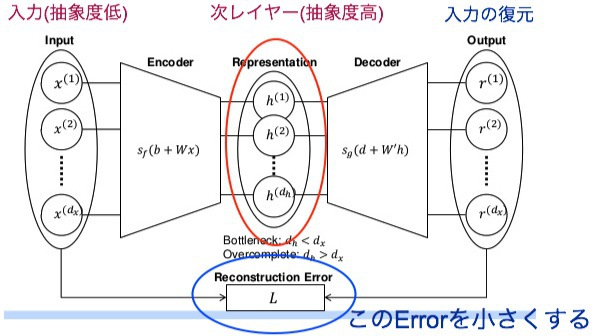
\includegraphics[width=80mm]{img/c3/autoencoder}
 \end{center}
 \caption{Autoencoderの構造図}
 \label{c3_autoencoder}
\end{figure}

\subsubsection{Denoising Autoencoder}
Denoising Autoencoderは、Autoencoderを拡張したものである。Input層に渡す入力データの一部をランダムに隠し(corrupted input)、元の隠されていない入力データを復元するように学習させる。データを隠す割合をcorruption rateといい、例えばcorruption rate30\%の場合、100次元の画像データだとしたら、そのうち30次元分をランダムに選んで、数値を0にしてしまうことになる。図\ref{c3_da_pic}は、Denoising Autoencoderが働く様子を、画像の入力レイヤーの場合について表している。\par
また、図\ref{c3_da}は、元の入力データ群から外れた入力データを作り、これを復元している様子を模式的に表している(\footnote{\url{http://www.iro.umontreal.ca/~bengioy/talks/icml2012-YB-tutorial.pdf}}より引用)。データの一部を隠すことによって、よりrobustな素性の作り方のモデルを得ることが出来ると考えられている。\par
なお、Denoising Autoencoderの学習過程には、Restricted Boltzman MachineのようなEnergy-Based Modelとの類似性があることがわかっている\cite{vincent2011a-connection}。
\begin{figure}[tbp]
 \begin{center}
  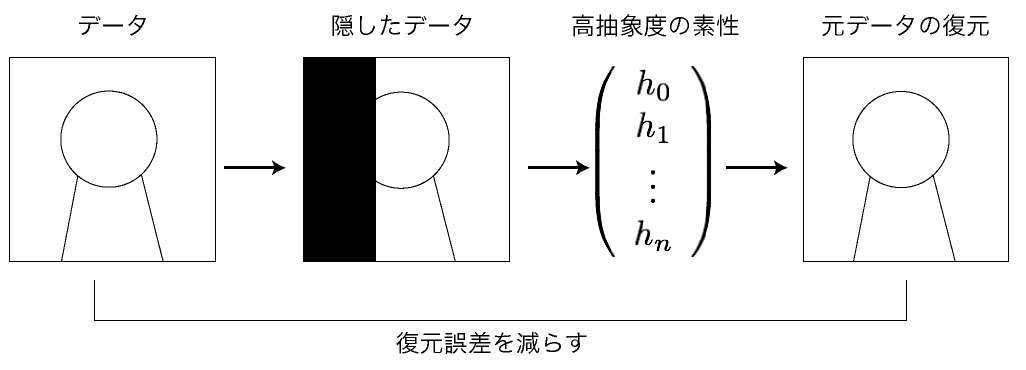
\includegraphics[width=80mm]{img/c3/da_pic}
 \end{center}
 \caption{画像に対するDenoising Autoencoder}
 \label{c3_da_pic}
\end{figure}

\begin{figure}[tbp]
 \begin{center}
  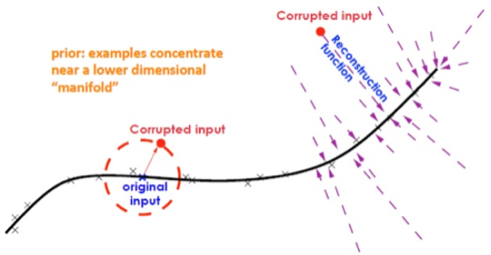
\includegraphics[width=80mm]{img/c3/da}
 \end{center}
 \caption{Denoising Autoencoderの模式図}
 \label{c3_da}
\end{figure}

\subsubsection{Stacked Denoising Autoencoder}
Stacked Denoising Autoencoder(SDA)は、Deep Belief Netsのpretrainingで、RBMの代わりにDenoising Autoencoder(以下DA)を用いたものである。DBN同様、前の層のRepresentationレイヤー = 次の層のInputレイヤーとなるように、DAで学習したレイヤーを積み重ねていく。最終レイヤーには、DAではなくSoftmaxレイヤーなどを置き、最終的な確率を出して、分類を行わせる。図\ref{c3_sda}は、SDAにて、どのようにpretrainingが繰り返され、DAが積み上げられていくのかを表している。いったんpretrainingが済んだら、そのレイヤーの入力は隠さず、学習された重みをそのまま使って高い抽象度の素性を作る。そして、その新しい素性を入力と捉えて、新たにDenoising Autoencoderの学習を行わせる。これを繰り返してレイヤーを積み上げ、最終的に良い素性を学習しやすいMLPを作ることで、finetuning段階でも学習がスムーズに進み、精度のよい推論ができるようになる。
\begin{figure}[tbp]
 \centering
  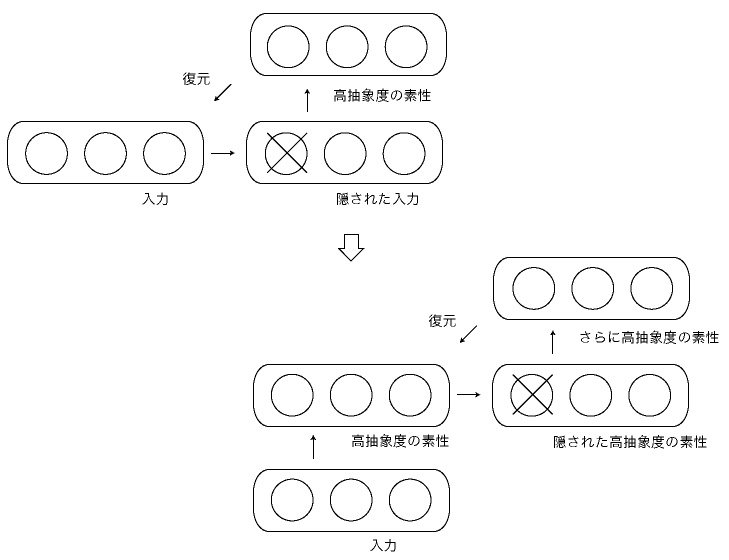
\includegraphics[width=100mm]{img/c3/sda}
 \caption{Stacked Denoising Autoencoderにおける学習の進行}
 \label{c3_sda}
\end{figure}

%Deep Learningの登場 Hinton, Bengio, LeCun
%画像認識タスクでの成績、音声認識タスクでの成果、猫認識
%MNIST, CIFAR, SVHNなどにおけるconv.net、Maxout, DropConnectの優位

\subsection{Convolutional Network}
Convolutional Network(畳み込みネットワーク)は、画像認識にて使われるニューラルネットワークの一種である。DBNやSDAのようにユニットが1対1で接続されるのではなく、画像上で距離が近いユニットを一まとめに考えるが特徴である。具体的には、フィルターと呼ばれる小さな四角形を、画像の上で動かしていき、フィルターが覆っている部分の性質を抽出して次のレイヤーに渡していく。フィルターは行列で表現されており、フィルター行列の各要素と、画像の各画素を掛け算し、その和を取ることで、次のレイヤーに渡す値が得られる。基本的な構造は、図\ref{c3_convolution}のようになっている。この図では、2回のconvolutionを行ったあと、十分に画像の素性が得られたところで、従来のMLPで見られる隠れレイヤーを1つ介して、出力を得ている。\par
\begin{figure}[tbp]
 \centering
  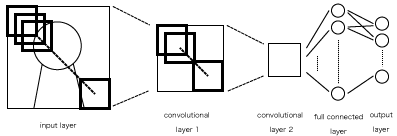
\includegraphics[width=80mm]{img/c3/convolution}
 \caption{Convolutional Netの仕組み}
 \label{c3_convolution}
\end{figure}
Convolutional Netの発祥はDBNやSDAよりも古い。画像上の各部分ごとに性質を抜き出しニューラルネットワークを構成するというアイデアは、人間の視覚野の仕組みを参考にしたもので、1980年のNeocognitronを始めとして\cite{fukushima1980neocognitron}\cite{fukushima1983neocognitron}様々な形で提唱されている\cite{lecun1998gradient-based}\cite{serre2007robust}。2003年に提唱されたConvolutional Netのモデルが、画像認識ベンチマークのMNISTにて、今でも5位の精度を保っており\cite{simard2003best}、2012年のものは2位となっている\cite{ciresan2012multi-column}。Fisherベクトルなど既存の画像認識手法との組み合わせでも、良い性能を発揮できることがわかっている\cite{nakayama2013efficient}。ここで紹介するのは、1998年にLeCunらが紹介した方法\cite{lecun1998gradient-based}であり、ほとんどのConvolutional Networkに使われているアルゴリズムの基本的な部分である。
\subsubsection{Feature Map}
実際のConvolutional Networkでは、Feature Mapと呼ばれる方法が使われている。これは、filterが1つだけでなく、複数種類のfilterを、複数枚の画像の上で動かしていく方法である。図\ref{c3_convolution}の構造に、Feature Mapの考え方を適用すると、\ref{c3_feature_map}のようになる。この図では、フィルターが移動する様子は省略している。四角形はFeature Map1つを、円はMLPのユニット1つを表している。Feature Map同士では、filterによる畳み込みによって情報が伝達される。Feature MapからMLPの隠れレイヤーにつながる部分では、まず全てのFeature Mapをつなげ、1次元のベクトルに並び替えて入力したと考えている。残りは、通常のMLPと同じように処理される。(なお、図\ref{c3_convolution}では、簡単のため、Feature Mapは表現されていない。)\par
1枚のmapが、1書類のfilterに対応しているので、filterの数と同じだけ次のレイヤーのFeature Mapが用意されている。それぞれのfilterを、全てのFeature Mapの上で動かして、畳み込み計算を行っていく。最終的に、普通のMLPに帰着させるところは変わらない。\par
Feature Mapは、カラー画像を扱うときにも利用できる。カラー画像データは、ほとんどの場合Red、Green、Blueの光の3原色に対応する3つの値にて表現される。これを省略してRGBと呼ぶ。Convolutional Netの入力レイヤーにて、画像サイズと同じ大きさの、RGBの3色に対応する3つのFeature Mapを設定することで、色情報を簡単に扱うことができる。

\begin{figure}[tbp]
 \centering
  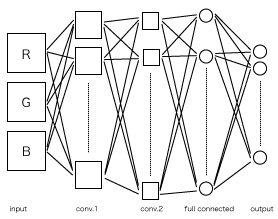
\includegraphics[width=80mm]{img/c3/feature_map}
 \caption{Convolutional Netとfeature map}
 \label{c3_feature_map}
\end{figure}

\subsubsection{Max-pooling}
Convolutinal Netにて、広く使われている方法のもう1つが、Max poolingである。Max pooling layerは普通Convolutional Layer同士の間に置かれる。Max poolingでは、convolutional layerで得られた画素を、部分ごとにたたみ込んでいく。ただし、convolutional layerの計算に使うfilterとは違い、重み行列は用いず、単純に対象領域の画素値のmaxを取って、次のレイヤーに渡していく。また、convolutional layerではfilterを1ピクセルずつ動かしていくが、max pooling layerでは、一度にfilterのサイズと同じだけ動かし、畳み込み対象領域が重ならないようにする。また、filterのサイズは2x2ピクセルに設定されることが多い。図\ref{c3_maxpooling}の左側は、max poolingによる畳み込みの様子を、右側ではMax-pooling Layerによる畳み込みの全体の様子を表している。\par
Max-poolingを用いることにより、各レイヤーの次元数を効率良く下げることが出来る。また同時に、ピクセルの位置が少し変化しても同じ結果が得られるので、位置的なrobustnessを上げることも出来る。\par
最後に、Max pooling Layerを用いた一般的なConvolutional Networkの全体図を、図\ref{c3_convnet}に挙げる。この図では、各Feature Mapごとのつながりは省略している。

\begin{figure}[tbp]
 \centering
  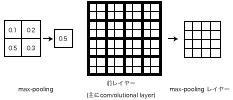
\includegraphics[width=80mm]{img/c3/maxpooling}
 \caption{Maxpoolingと、Maxpooling Layerの作用}
 \label{c3_maxpooling}
\end{figure}

\begin{figure}[tbp]
 \centering
  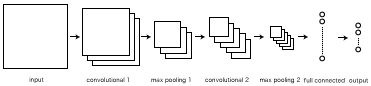
\includegraphics[width=120mm]{img/c3/convnet}
 \caption{max pooling layerを取り入れたConvolutional Network}
 \label{c3_convnet}
\end{figure}

\subsection{DropoutとDropConnect}
\label{c3_dropout}
Dropoutとは、2012年にHinton氏らによって提案された、過学習を防ぐための技術である\cite{hinton2012improving}。過学習とは、機械学習全般において使われる用語で、学習モデルが訓練中に見たデータへの適応を重視し過ぎたために、未知のデータをうまく識別できなくなる現象のことを指す。Dropoutでは、過学習を防ぐため、各レイヤーからの出力をランダムに消去してしまう。これによって各ユニットには、他のユニットに頼らず自力で学習をする必要が生じ、より様々な入力に対応しやすい堅固(robust)なモデルが獲得される、と考えられている。図\ref{c3_dropout_timit}は、\cite{hinton2012improving}より引用した図で、音声認識のTIMITデータベース\cite{fisher1986darpa}\footnote{\url{http://catalog.ldc.upenn.edu/LDC93S1}}に対する識別精度である。Dropoutを使うことで、使わなかった場合に比べ、特にEpoch数(学習の繰り返し回数)が大きい場合に分類精度が向上していることがわかる。\par
DropConnectは、Dropoutをさらに一般化した手法である。DropConnectでは、各ユニットからの出力ではなく、ユニット同士のつながりをランダムにカットしている。図\ref{c3_dropconnect}は、DropConnectの著者による紹介Webページ\footnote{\url{http://cs.nyu.edu/~wanli/dropc/}}に掲載されている画像の引用である。ニューラルネットワークにおけるニューロン同士の接続が、ランダムに切断されている様子を表している。
\begin{figure}[tbp]
 \begin{center}
  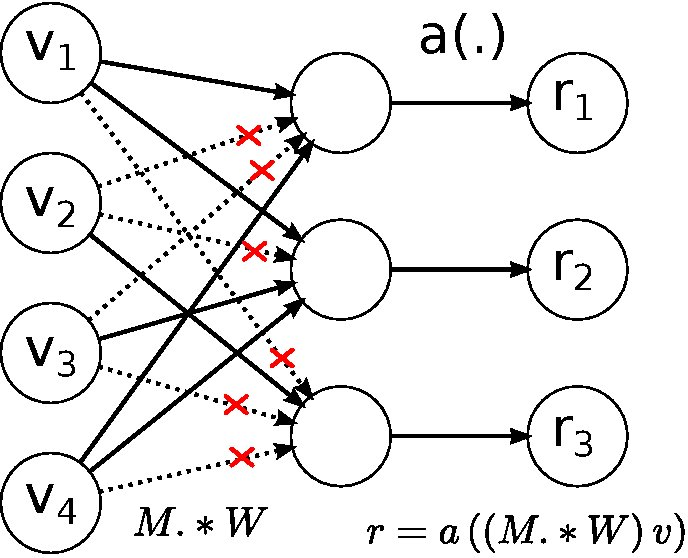
\includegraphics[width=50mm]{img/c3/nn_dc}
 \end{center}
 \caption{DropConnectの模式図}
 \label{c3_dropconnect}
\end{figure}

\subsection{活性化関数}
各ユニットに入力された値は、ある一定の関数によって増幅・変換される。これは人間の神経細胞を真似た仕組みで、神経細胞の化学物質による活性化にちなんで、活性化関数(activation function)と呼ばれる。この項では、ニューラルネットにおける様々な活性化関数を紹介する。
\subsubsection{heaviside関数}
始めにニューラルネットワークの活性化関数として用いられたがHeavisideの階段関数である。この関数は負値に0、正値に1を返す。数式では、
\begin{equation}
H(x)= \left\{\begin{array}{cc} 0\quad (x < 0)\\ 1 \quad (x > 0)\end{array}\right.
\end{equation}
となる。ただし、これだけでは$x=0$の点で不連続になるので、$H(x)=0$や$H(x)=0.5$などの定義が用いられる。ヘビサイド関数のグラフを\ref{c3_heaviside}に示す。\par
heaviside関数は、ニューロンが受けた刺激の総和を測り、閾値を超えていれば次のニューロンにも情報を伝達し、超えていなければ何もしないという性質をそのまま反映している。しかし、この関数は微分不可能なため、バックプロパゲーションを行う上では不都合であり、特にDeep Learningのネットワークモデルにおいて使われることは少ない。
\begin{figure}[tbp]
 \centering
  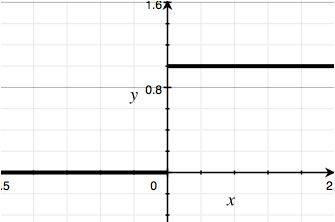
\includegraphics[width=80mm]{img/c3/heaviside}
 \caption{Heavisideの階段関数}
 \label{c3_heaviside}
\end{figure}

\subsubsection{sigmoid関数とhyperbolic tangent}
シグモイド関数は、ヘビサイド関数に似ているが、全域にて非線形かつ微分可能である。この2つの特性により、バックプロパゲーションに適している。以下の式で表される。
\begin{equation}
S(x) = \frac{1}{1+e^{-x}}
\end{equation}
また、微分した形が同じシグモイド関数で表されるという特徴があり、実装が容易である。
\begin{eqnarray}
\frac{d}{dx}S(x) &=& \left( \frac{1}{1+e^{-x}} \right) \left( \frac{-e^{-x}}{1+e^{-x}} \right)\\
&=& S(x)(1-S(x))
\end{eqnarray}
シグモイド関数のグラフが図\ref{c3_sigmoid}である。Heaviside関数を$x=0$の付近のみ滑らかにしたような形をしている。この関数は、xの絶対値が大きくなるにつれ、yの変化が非常にに小さくなっている。そのため、ユニット間伝達において、入力と重みの積が大きくなってしまうと、その部分は誤差のバックプロパゲーションに対する反応が小さくなってしまい、学習が進みにくくなってしまうという弱点がある。
\begin{figure}[tbp]
 \centering
  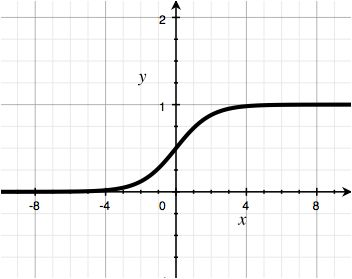
\includegraphics[width=80mm]{img/c3/sigmoid}
 \caption{Sigmoid関数}
 \label{c3_sigmoid}
\end{figure}
なお、hyperbolic tangent関数、通称tanh関数を用いることもある。sigmoid関数とtanh関数は線形の差しかないため、ニューラルネットワークの性能という面では、どちらを使用しても等価である。
\begin{equation}
tanh(x) = \frac{e^x-e^{-x}}{e^x+e^{-x}} \\\\
\end{equation}
\begin{equation}
S(x) = \frac{tanh(x/2)+1}{2}
\end{equation}

\subsubsection{Rectifier Unit}
Rectifier関数は、最近のニューラルネットワークにおいてよく用いられている活性化関数である。
\begin{equation}
f(x) = max(0, x) = \left\{\begin{array}{cc} 0\quad (x < 0)\\ x \quad (x > 0)\end{array}\right.
\end{equation}
Rectifier関数が性能向上に役立つ理由は、まだ解明されていない。

\begin{figure}[tbp]
 \centering
  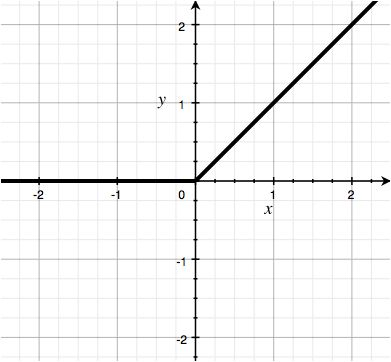
\includegraphics[width=80mm]{img/c3/rectifier}
 \caption{Rectifier関数}
 \label{c3_rectifier}
\end{figure}

\subsubsection{Maxout Unit}
Maxout Networkとは、バックプロパゲーションを伴う単純な多層MLP構造に、\ref{c3_dropout}で述べたDropout法を組み合わせ、さらにMaxout Unitという特殊な活性化関数を併用したニューラルネットワークである\cite{goodfellow2013maxout}。Maxout Networkの1レイヤー分の構造を、図\ref{c3_maxout_arch}に示す。\par
Maxout Unitでは、複数の線形ユニットの出力について、maxを取っている。これにより、任意の凸関数を近似することが出来る。図\ref{c3_maxout_app}は、Maxout Unitが凸関数を近似する様子を、1次元の入力について示している。そして、複数のmaxout unitの線形和を取ることは、複数の近似された凸関数の線形和を取ることである。これによって、最終的に任意の連続関数を近似できることが証明されている。
\begin{figure}[tbp]
 \begin{center}
  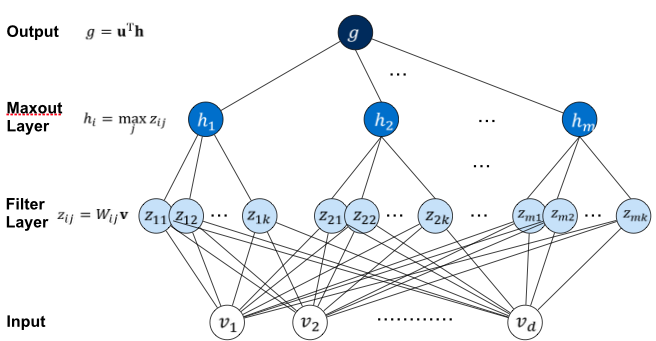
\includegraphics[width=100mm]{img/c3/maxout_arch}
 \end{center}
 \caption{Maxout Networkの構造図}
 \label{c3_maxout_arch}
\end{figure}
\begin{figure}[tbp]
 \begin{center}
  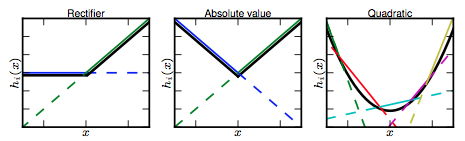
\includegraphics[width=100mm]{img/c3/maxout_app}
 \end{center}
 \caption{Maxout Unitが凸関数を近似する様子(1次元の場合)}
 \label{c3_maxout_app}
\end{figure}
